\documentclass{article}
% generated by Madoko, version 1.0.3
%mdk-data-line={1}


\usepackage[heading-base={2},section-num={False},bib-label={True}]{madoko2}


\begin{document}



\mdxtitleblockstart{}
\mdxtitle{MASSIVE DATA PROCESSING 
               ( Ecole Centrale)}%mdk

\mdxsubtitle{ASSIGNMENT 1 - HADOOP}%mdk
\mdxauthorstart{}
\mdxauthorname{Raunaq Paul}%mdk
\mdxauthorend\mdtitleauthorrunning{}{}\mdxtitleblockend%mdk

\section{1.\hspace*{0.5em}OBJECTIVE}\label{heading}%mdk%mdk

\noindent The objective of the assignment is to get used to working with Haddoop Framework and execute wordcount and map reduce jobs on given text files.
The following are the questions answered  in this assignment:%mdk

We are asked to implement an inverted index in MapReduce for the document corpus of pg100.txt (from http://www.gutenberg.org/cache/epub/100/pg100.txt), pg31100.txt (from http://www.gutenberg.org/cache/epub/31100/pg31100.txt) and pg3200.txt (from http://www.gutenberg.org/cache/epub/3200/pg3200.txt). This corpus includes the complete works of William Shakespear, Mark Twain and Jane Austen, respectively.%mdk

An inverted index (also referred to as postings file or inverted file) is an index data structure storing a mapping from content, such as words or numbers, to its locations in a database file, or in a document or a set of documents.The purpose of an inverted index is to allow fast full text searches, at a cost of increased processing when a document is added to the database. The inverted file may be the database file itself, rather than its index. It is the most popular data structure used in document retrieval systems,used on a large scale for example in search engines.%mdk

It provides for each distinct word in a document corpus, the filenames that contain this word, along with some other information (e.g., count/position within each document).%mdk

For example, assume you are given the following corpus, consisting of doc1.txt, doc2.txt and doc3.txt:%mdk

\begin{itemize}[noitemsep,topsep=\mdcompacttopsep]%mdk

\item doc1.txt: “This is a very useful program. It is also quite easy.”%mdk

\item doc2.txt: “This is my first MapReduce program.”%mdk

\item doc3.txt: “Its result is an inverted index.”%mdk
%mdk
\end{itemize}%mdk

\noindent An inverted index would contain the following data (in random order):%mdk
\begin{mdtabular}{2}{\dimeval{(\linewidth)/2}}{1ex}%mdk
\begin{tabular}{lc}\midrule
\multicolumn{1}{|c}{{\bfseries Word}}&\multicolumn{1}{c|}{{\bfseries FileName}}\\

\midrule
\multicolumn{1}{|l}{this}&\multicolumn{1}{c|}{doc1.txt, doc2.txt}\\
\multicolumn{1}{|l}{is}&\multicolumn{1}{c|}{doc1.txt, doc2.txt, doc3.txt}\\
\multicolumn{1}{|l}{a}&\multicolumn{1}{c|}{doc1.txt}\\
\multicolumn{1}{|l}{program}&\multicolumn{1}{c|}{doc1.txt, doc2.txt}\\
\midrule
\end{tabular}\end{mdtabular}

\noindent Before the inverted index, we will also be executing wordcount jobs in order to find StopWords or frequently appearing words which do not affect the content of the documents much e.g. articles.%mdk

\section{2.\hspace*{0.5em}Initialization}\label{heading}%mdk%mdk

\noindent First we create a new workspace called MDP\_Assignment1 from the Cloudera Terminal. Then, we create an input and output directory in our workspace:%mdk
\begin{mdpre}%mdk
\noindent cd~workspace/InvertedIndex\\
mkdir~input\\
mkdir~output\\
%mdk
\end{mdpre}\noindent We then download the text files and put the, in the input directory of our MDP\_Assignment1 workspace.
We can now put the input text files into Hadoop:
\begin{mdpre}%mdk
\noindent{}[cloudera@quickstart~\textasciitilde{}]\$~cd~workspace/MDP\_Assignment1\\
{}[cloudera@quickstart~MDP\_Assignment1]\$~hadoop~fs~-mkdir~input\\
{}[cloudera@quickstart~MDP\_Assignment1]\$~hadoop~fs~-put~input/pg100.txt~input\\
{}[cloudera@quickstart~MDP\_Assignment1]\$~hadoop~fs~-put~input/pg3200.txt~input\\
{}[cloudera@quickstart~MDP\_Assignment1]\$~hadoop~fs~-put~input/pg31100.txt~input\\
{}[cloudera@quickstart~MDP\_Assignment1]\$~hadoop~fs~-ls~input\\
Found~{\mdcolor{purple}3}~items\\
-rw-r--r--~~~{\mdcolor{purple}1}~cloudera~cloudera~~~~{\mdcolor{purple}5589917}~{\mdcolor{purple}2017}-{\mdcolor{purple}02}-{\mdcolor{purple}16}~{\mdcolor{purple}05}:{\mdcolor{purple}09}~input/pg100.txt\\
-rw-r--r--~~~{\mdcolor{purple}1}~cloudera~cloudera~~~~{\mdcolor{purple}4454075}~{\mdcolor{purple}2017}-{\mdcolor{purple}02}-{\mdcolor{purple}16}~{\mdcolor{purple}05}:{\mdcolor{purple}11}~input/pg31100.txt\\
-rw-r--r--~~~{\mdcolor{purple}1}~cloudera~cloudera~~~{\mdcolor{purple}16013958}~{\mdcolor{purple}2017}-{\mdcolor{purple}02}-{\mdcolor{purple}16}~{\mdcolor{purple}05}:{\mdcolor{purple}10}~input/pg3200.txt\\
%mdk
\end{mdpre}\noindent We are now ready to start creating our jobs for the assignment.

\subsection{2.1.\hspace*{0.5em}Question: StopWords}\label{heading}%mdk%mdk

\noindent\textbf{Run a MapReduce program to identify stop words(words with frequency \textgreater{} 4000) 
for   the given   document   corpus. Store   them   in   a   single   csv   file   on   HDFS
(stopwords.csv).
You can edit the several parts of the reducers’ output after the job 
finishes (with hdfs commands or with a text editor), in order to merge them as a single 
csv file.}%mdk

We will now implement our map reduce program. We will try to find the stopwords in our corpus by finding 
the wordcounts for the entire corpus first and then separating the words with frequency \textgreater{} 4000 a \textquotedblleft{}stopwords\textquotedblright{} by adding the condition.%mdk

For this, we reused the code from Standford http://snap.stanford.edu/class/cs246-data-2014/WordCount.java given in the CS246: Mining Massive Datasets Hadoop tutorial.%mdk
\begin{mdpre}%mdk
\noindent{\mdcolor{navy}package}~edu.stanford.cs246.wordcount;\\
\\
{\mdcolor{navy}import}~java.io.IOException;\\
{\mdcolor{navy}import}~java.util.Arrays;\\
{\mdcolor{navy}import}~org.apache.hadoop.conf.Configuration;\\
{\mdcolor{navy}import}~org.apache.hadoop.conf.Configured;\\
{\mdcolor{navy}import}~org.apache.hadoop.fs.Path;\\
{\mdcolor{navy}import}~org.apache.hadoop.io.IntWritable;\\
{\mdcolor{navy}import}~org.apache.hadoop.io.LongWritable;\\
{\mdcolor{navy}import}~org.apache.hadoop.io.Text;\\
{\mdcolor{navy}import}~org.apache.hadoop.mapreduce.Job;\\
{\mdcolor{navy}import}~org.apache.hadoop.mapreduce.Mapper;\\
{\mdcolor{navy}import}~org.apache.hadoop.mapreduce.Reducer;\\
{\mdcolor{navy}import}~org.apache.hadoop.mapreduce.lib.input.FileInputFormat;\\
{\mdcolor{navy}import}~org.apache.hadoop.mapreduce.lib.input.TextInputFormat;\\
{\mdcolor{navy}import}~org.apache.hadoop.mapreduce.lib.output.FileOutputFormat;\\
{\mdcolor{navy}import}~org.apache.hadoop.mapreduce.lib.output.TextOutputFormat;\\
{\mdcolor{navy}import}~org.apache.hadoop.util.Tool;\\
{\mdcolor{navy}import}~org.apache.hadoop.util.ToolRunner;\\
\\
{\mdcolor{navy}public}~{\mdcolor{navy}class}~WordCount~{\mdcolor{navy}extends}~Configured~{\mdcolor{navy}implements}~Tool~\{\\
~~~{\mdcolor{navy}public}~{\mdcolor{navy}static}~{\mdcolor{navy}void}~main(String{}[]~args)~{\mdcolor{navy}throws}~Exception~\{\\
~~~~~~System.out.println(Arrays.{\mdcolor{navy}toString}(args));\\
~~~~~~{\mdcolor{navy}int}~res~=~ToolRunner.run({\mdcolor{navy}new}~Configuration(),~{\mdcolor{navy}new}~WordCount(),~args);\\
~~~~~~\\
~~~~~~System.exit(res);\\
~~~\}\\
\\
~~~@Override\\
~~~{\mdcolor{navy}public}~{\mdcolor{navy}int}~run(String{}[]~args)~{\mdcolor{navy}throws}~Exception~\{\\
~~~~~~System.out.println(Arrays.{\mdcolor{navy}toString}(args));\\
~~~~~~Job~job~=~{\mdcolor{navy}new}~Job(getConf(),~{\mdcolor{maroon}"}{\mdcolor{maroon}WordCount}{\mdcolor{maroon}"});\\
~~~~~~job.setJarByClass(WordCount.{\mdcolor{navy}class});\\
~~~~~~job.setOutputKeyClass(Text.{\mdcolor{navy}class});\\
~~~~~~job.setOutputValueClass(IntWritable.{\mdcolor{navy}class});\\
\\
~~~~~~job.setMapperClass(Map.{\mdcolor{navy}class});\\
~~~~~~job.setReducerClass(Reduce.{\mdcolor{navy}class});\\
\\
~~~~~~job.setInputFormatClass(TextInputFormat.{\mdcolor{navy}class});\\
~~~~~~job.setOutputFormatClass(TextOutputFormat.{\mdcolor{navy}class});\\
\\
~~~~~~FileInputFormat.addInputPath(job,~{\mdcolor{navy}new}~Path(args{}[{\mdcolor{purple}0}]));\\
~~~~~~FileOutputFormat.setOutputPath(job,~{\mdcolor{navy}new}~Path(args{}[{\mdcolor{purple}1}]));\\
\\
~~~~~~job.waitForCompletion({\mdcolor{navy}true});\\
~~~~~~\\
~~~~~~{\mdcolor{navy}return}~{\mdcolor{purple}0};\\
~~~\}\\
~~~\\
~~~{\mdcolor{navy}public}~{\mdcolor{navy}static}~{\mdcolor{navy}class}~Map~{\mdcolor{navy}extends}~Mapper\textless{}LongWritable,~Text,~Text,~IntWritable\textgreater{}~\{\\
~~~~~~{\mdcolor{navy}private}~{\mdcolor{navy}final}~{\mdcolor{navy}static}~IntWritable~ONE~=~{\mdcolor{navy}new}~IntWritable({\mdcolor{purple}1});\\
~~~~~~{\mdcolor{navy}private}~Text~word~=~{\mdcolor{navy}new}~Text();\\
\\
~~~~~~@Override\\
~~~~~~{\mdcolor{navy}public}~{\mdcolor{navy}void}~map(LongWritable~key,~Text~value,~Context~context)\\
~~~~~~~~~~~~~~{\mdcolor{navy}throws}~IOException,~InterruptedException~\{\\
~~~~~~~~~{\mdcolor{navy}for}~(String~token:~value.{\mdcolor{navy}toString}().split({\mdcolor{maroon}"}{\mdcolor{gray}\textbackslash{}\textbackslash{}}{\mdcolor{maroon}s+}{\mdcolor{maroon}"}))~\{\\
~~~~~~~~~~~~word.set(token);\\
~~~~~~~~~~~~context.write(word,~ONE);\\
~~~~~~~~~\}\\
~~~~~~\}\\
~~~\}\\
\\
~~~{\mdcolor{navy}public}~{\mdcolor{navy}static}~{\mdcolor{navy}class}~Reduce~{\mdcolor{navy}extends}~Reducer\textless{}Text,~IntWritable,~Text,~IntWritable\textgreater{}~\{\\
~~~~~~@Override\\
~~~~~~{\mdcolor{navy}public}~{\mdcolor{navy}void}~reduce(Text~key,~Iterable\textless{}IntWritable\textgreater{}~values,~Context~context)\\
~~~~~~~~~~~~~~{\mdcolor{navy}throws}~IOException,~InterruptedException~\{\\
~~~~~~~~~{\mdcolor{navy}int}~sum~=~{\mdcolor{purple}0};\\
~~~~~~~~~{\mdcolor{navy}for}~(IntWritable~val~:~values)~\{\\
~~~~~~~~~~~~sum~+=~val.get();\\
~~~~~~~~~\}\\
~~~~~~~~~context.write(key,~{\mdcolor{navy}new}~IntWritable(sum));\\
~~~~~~\}\\
~~~\}\\
\}\\
%mdk
\end{mdpre}\noindent The changes made to the above code are as follows: 

\begin{itemize}%mdk

\item{}
Added the following code to the Main Class ( Driver):%mdk
\begin{mdpre}%mdk
\noindent job.getConfiguration().set({\mdcolor{maroon}"}{\mdcolor{maroon}mapreduce.output.textoutputformat.separator}{\mdcolor{maroon}"},~{\mdcolor{maroon}"}{\mdcolor{maroon},}{\mdcolor{maroon}"});%mdk
\end{mdpre}
The above code creates our output in the form of a csv format as needed per the task.%mdk%mdk

\item{}
toLowerCase() method and replaceAll(\textquotedblleft{}{}[\textasciicircum{}a-zA-Z ]\textquotedblright{}, \textquotedblleft{}\textquotedblright{}) in the words iteration in the Mapper function in order to remove redundancy/duplicates and only have alphabetical outputs:%mdk%mdk
%mdk
\end{itemize}%mdk
\begin{mdpre}%mdk
\noindent{\mdcolor{navy}public}~{\mdcolor{navy}static}~{\mdcolor{navy}class}~StubMapper~{\mdcolor{navy}extends}~Mapper\textless{}LongWritable,~Text,~Text,~IntWritable\textgreater{}\\
~~~~\{\\
~~~~~~~~~~~~~~~~~{\mdcolor{navy}private}~{\mdcolor{navy}final}~{\mdcolor{navy}static}~IntWritable~ONE~=~{\mdcolor{navy}new}~IntWritable({\mdcolor{purple}1});\\
~~~~~~~~~~~~~~~~~{\mdcolor{navy}private}~Text~word~=~{\mdcolor{navy}new}~Text();\\
\\
~~~~~~~~~~~~~@Override\\
~~~~~~~~~~~~~~{\mdcolor{navy}public}~{\mdcolor{navy}void}~map(LongWritable~key,~Text~value,~Context~context)\\
~~~~~~~~~~~~~~~~~~{\mdcolor{navy}throws}~IOException,~InterruptedException~\\
~~~~~~~~~~~~~\{\\
~~~~~~~~~~~~~~~~~~~~~~~~~~~~~~~~{\mdcolor{navy}for}~(String~token~:~value.{\mdcolor{navy}toString}().replaceAll({\mdcolor{maroon}"}{\mdcolor{maroon}{}[\textasciicircum{}a-zA-Z~]}{\mdcolor{maroon}"},~{\mdcolor{maroon}"}{\mdcolor{maroon}"}).split({\mdcolor{maroon}"}{\mdcolor{gray}\textbackslash{}\textbackslash{}}{\mdcolor{maroon}s+}{\mdcolor{maroon}"}))~\\
~~~~~~~~~~~~~~~~~~~~~~~~~~~~~~~~\{\\
~~~~~~~~~~~~~~~~~~~~~~~~~~~~~~~~~~~word.set(token.toLowerCase());\\
~~~~~~~~~~~~~~~~~~~~~~~~~~~~~~~~~~~context.write(word,~ONE);\\
~~~~~~~~~~~~~~~~~~~~~~~~~~~~~~~~\}\\
~~~~~~~~~~~~~\}\\
~~~~~~~~\}%mdk
\end{mdpre}
\begin{itemize}[noitemsep,topsep=\mdcompacttopsep]%mdk

\item if statement in the Reducer class that selects only the stopwords ( words with Frequency\textgreater{}4000),
before writing the (key,value) outputs:%mdk
%mdk
\end{itemize}%mdk
\begin{mdpre}%mdk
\noindent{\mdcolor{navy}public}~{\mdcolor{navy}static}~{\mdcolor{navy}class}~StubReducer~{\mdcolor{navy}extends}~Reducer\textless{}Text,~IntWritable,~Text,~IntWritable\textgreater{}\\
~~~~\{\\
~~~~~~~~~~~~~~~~~@Override\\
~~~~~~~~~~~~~~~~~~~~{\mdcolor{navy}public}~{\mdcolor{navy}void}~reduce(Text~key,~Iterable\textless{}IntWritable\textgreater{}~values,Context~context)~{\mdcolor{navy}throws}~IOException,~InterruptedException~\\
~~~~~~~~~~~~~~~~~\{\\
~~~~~~~~~~~~~~~~~~~~~~~~~~~~~~~~~~~~~~~~~{\mdcolor{navy}int}~sum~=~{\mdcolor{purple}0};\\
~~~~~~~~~~~~~~~~~~~~~~~~~~~~~~~~~~~~~~~~~{\mdcolor{navy}for}~(IntWritable~val~:~values)~\\
~~~~~~~~~~~~~~~~~~~~~~~~~~~~~~~~~~~~~~~~~~~~~~~~~\{\\
~~~~~~~~~~~~~~~~~~~~~~~~~~~~~~~~~~~~~~~~~~~~~~~~~~~sum~+=~val.get();\\
~~~~~~~~~~~~~~~~~~~~~~~~~~~~~~~~~~~~~~~~~~~~~~~~~\}\\
~~~~~~~~~~~~~~~~~~~~~~~~~~~~~~~~~~~~~~~~~{\mdcolor{navy}if}~(sum~\textgreater{}~{\mdcolor{purple}4000})~\\
~~~~~~~~~~~~~~~~~~~~~~~~~~~~~~~~~~~~~~~~~~\{\\
~~~~~~~~~~~~~~~~~~~~~~~~~~~~~~~~~~~~~~~~~~~~~context.write(key,~{\mdcolor{navy}new}~IntWritable(sum));\\
~~~~~~~~~~~~~~~~~~~~~~~~~~~~~~~~~~~~~~~~~~\}\\
~~~~~~~~~~~~~~~~~\}\\
\\
~~~~\}%mdk
\end{mdpre}\noindent After this , we execute the code and export the Jar file and run it using the following hadoop job code:
\begin{mdpre}%mdk
\noindent hadoop~jar~MDP\_Assignment1.jar~stopwords.stopwords~input~output%mdk
\end{mdpre}\noindent We can now see the results located in the HDFS output directory by using the following command in the terminal:
\begin{mdpre}%mdk
\noindent hadoop~fs~-ls~output\\
Found~{\mdcolor{purple}2}~items\\
-rw-r--r--~~~{\mdcolor{purple}1}~cloudera~cloudera~~~~~~~~~~{\mdcolor{purple}0}~{\mdcolor{purple}2017}-{\mdcolor{purple}02}-{\mdcolor{purple}16}~{\mdcolor{purple}05}:{\mdcolor{purple}14}~output/\_SUCCESS\\
-rw-r--r--~~~{\mdcolor{purple}1}~cloudera~cloudera~~~~~~~{\mdcolor{purple}1333}~{\mdcolor{purple}2017}-{\mdcolor{purple}02}-{\mdcolor{purple}16}~{\mdcolor{purple}05}:{\mdcolor{purple}14}~output/part-r-{\mdcolor{purple}00000}\\
%mdk
\end{mdpre}\noindent We now Merge the output file to the output folder in our workspace/MDP\_Assignment into stopwords.csv
\begin{mdpre}%mdk
\noindent hadoop~fs~-getmerge~output~output/stopwords.csv\\
%mdk
\end{mdpre}\noindent The stopwords.csv is in the following format:
\begin{mdpre}%mdk
\noindent a,{\mdcolor{purple}100360}\\
about,{\mdcolor{purple}7928}\\
after,{\mdcolor{purple}4651}\\
again,{\mdcolor{purple}4900}\\
all,{\mdcolor{purple}21349}\\
am,{\mdcolor{purple}6747}%mdk
\end{mdpre}\noindent The following is the log execution time which can be seen in the Hadoop Yarn Resource Manager: 

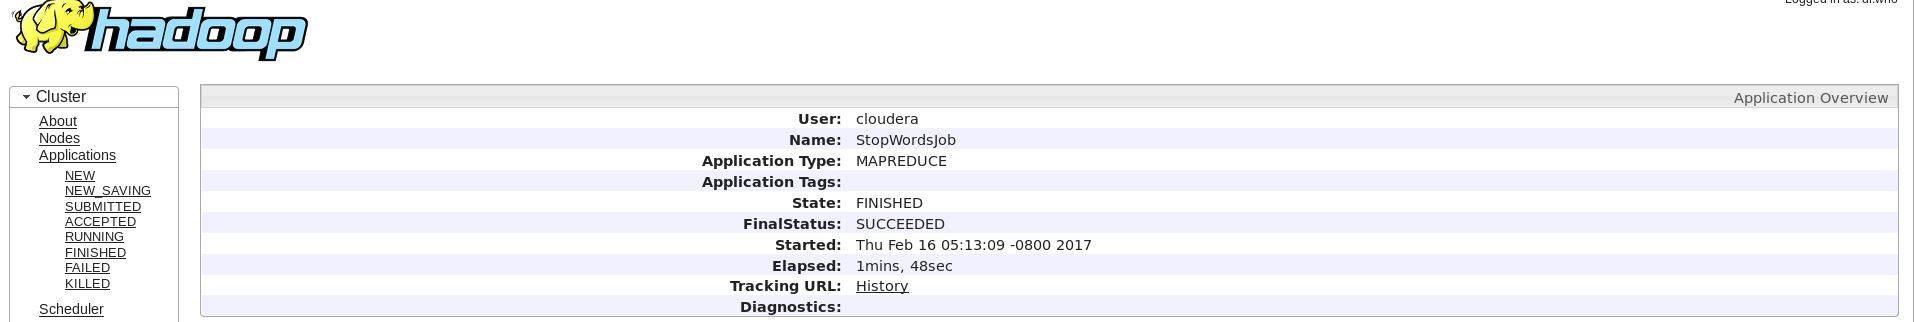
\includegraphics[keepaspectratio=true,width=\dimmin{}{\dimwidth{1.30}}]{images/16763454_10208853135827919_2062444645_o}{}%mdk

\noindent Now we answer the following questions as per the tasks:%mdk

\subsubsection{2.1.1.\hspace*{0.5em}Use  10 reducers and do not use a combiner. Report the execution time.}\label{heading}%mdk%mdk

\noindent The number of reducers is defined in the Hadoop driver configuration (main class) by the method:
job.setNumReduceTasks().
In this case, we use:
job.getConfiguration().set(\textquotedblleft{}mapreduce.output.textoutputformat.separator\textquotedblright{}, \textquotedblleft{},\textquotedblright{});
        job.setNumReduceTasks(10);%mdk

The following is the Hadoop Job code in the terminal:%mdk
\begin{mdpre}%mdk
\noindent hadoop~jar~MDP\_Assignment1.jar~stopwords.stopwords2~input~output\\
hadoop~fs~-ls~output\\
Found~{\mdcolor{purple}11}~items\\
-rw-r--r--~~~{\mdcolor{purple}1}~cloudera~cloudera~~~~~~~~~~{\mdcolor{purple}0}~{\mdcolor{purple}2017}-{\mdcolor{purple}02}-{\mdcolor{purple}16}~{\mdcolor{purple}05}:{\mdcolor{purple}46}~output/\_SUCCESS\\
-rw-r--r--~~~{\mdcolor{purple}1}~cloudera~cloudera~~~~~~~~{\mdcolor{purple}100}~{\mdcolor{purple}2017}-{\mdcolor{purple}02}-{\mdcolor{purple}16}~{\mdcolor{purple}05}:{\mdcolor{purple}45}~output/part-r-{\mdcolor{purple}00000}\\
-rw-r--r--~~~{\mdcolor{purple}1}~cloudera~cloudera~~~~~~~~{\mdcolor{purple}219}~{\mdcolor{purple}2017}-{\mdcolor{purple}02}-{\mdcolor{purple}16}~{\mdcolor{purple}05}:{\mdcolor{purple}45}~output/part-r-{\mdcolor{purple}00001}\\
-rw-r--r--~~~{\mdcolor{purple}1}~cloudera~cloudera~~~~~~~~{\mdcolor{purple}160}~{\mdcolor{purple}2017}-{\mdcolor{purple}02}-{\mdcolor{purple}16}~{\mdcolor{purple}05}:{\mdcolor{purple}45}~output/part-r-{\mdcolor{purple}00002}\\
-rw-r--r--~~~{\mdcolor{purple}1}~cloudera~cloudera~~~~~~~~{\mdcolor{purple}121}~{\mdcolor{purple}2017}-{\mdcolor{purple}02}-{\mdcolor{purple}16}~{\mdcolor{purple}05}:{\mdcolor{purple}45}~output/part-r-{\mdcolor{purple}00003}\\
-rw-r--r--~~~{\mdcolor{purple}1}~cloudera~cloudera~~~~~~~~~{\mdcolor{purple}68}~{\mdcolor{purple}2017}-{\mdcolor{purple}02}-{\mdcolor{purple}16}~{\mdcolor{purple}05}:{\mdcolor{purple}45}~output/part-r-{\mdcolor{purple}00004}\\
-rw-r--r--~~~{\mdcolor{purple}1}~cloudera~cloudera~~~~~~~~{\mdcolor{purple}138}~{\mdcolor{purple}2017}-{\mdcolor{purple}02}-{\mdcolor{purple}16}~{\mdcolor{purple}05}:{\mdcolor{purple}45}~output/part-r-{\mdcolor{purple}00005}\\
-rw-r--r--~~~{\mdcolor{purple}1}~cloudera~cloudera~~~~~~~~{\mdcolor{purple}139}~{\mdcolor{purple}2017}-{\mdcolor{purple}02}-{\mdcolor{purple}16}~{\mdcolor{purple}05}:{\mdcolor{purple}46}~output/part-r-{\mdcolor{purple}00006}\\
-rw-r--r--~~~{\mdcolor{purple}1}~cloudera~cloudera~~~~~~~~{\mdcolor{purple}139}~{\mdcolor{purple}2017}-{\mdcolor{purple}02}-{\mdcolor{purple}16}~{\mdcolor{purple}05}:{\mdcolor{purple}46}~output/part-r-{\mdcolor{purple}00007}\\
-rw-r--r--~~~{\mdcolor{purple}1}~cloudera~cloudera~~~~~~~~{\mdcolor{purple}182}~{\mdcolor{purple}2017}-{\mdcolor{purple}02}-{\mdcolor{purple}16}~{\mdcolor{purple}05}:{\mdcolor{purple}46}~output/part-r-{\mdcolor{purple}0000}{\mdcolor{purple}8}\\
-rw-r--r--~~~{\mdcolor{purple}1}~cloudera~cloudera~~~~~~~~~{\mdcolor{purple}67}~{\mdcolor{purple}2017}-{\mdcolor{purple}02}-{\mdcolor{purple}16}~{\mdcolor{purple}05}:{\mdcolor{purple}46}~output/part-r-{\mdcolor{purple}0000}{\mdcolor{purple}9}\\
hadoop~fs~-getmerge~output~output/stopwords2.csv\\
%mdk
\end{mdpre}\noindent The csv file stopwords2 consists of all words except the ones in stopwords.csv
\begin{mdpre}%mdk
\noindent about,{\mdcolor{purple}7928}\\
be,{\mdcolor{purple}28477}\\
before,{\mdcolor{purple}5630}\\
by,{\mdcolor{purple}20273}\\
her,{\mdcolor{purple}28370}%mdk
\end{mdpre}\noindent Execution Time:

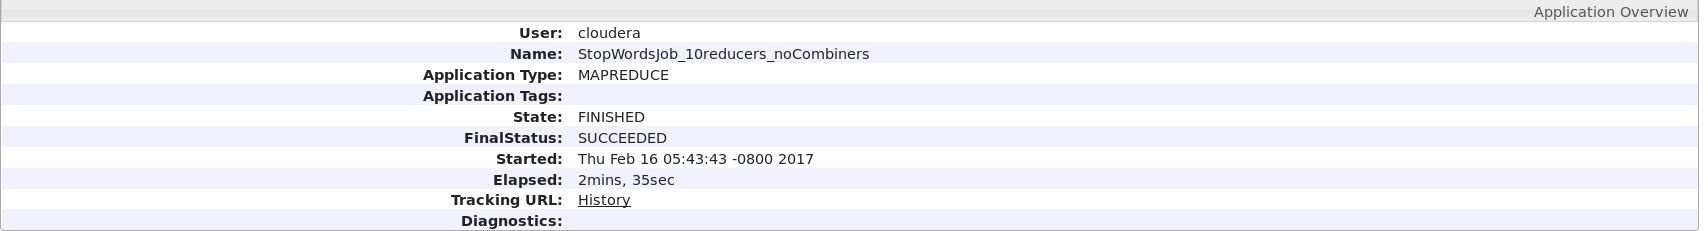
\includegraphics[keepaspectratio=true,width=\dimmin{}{\dimwidth{1.30}}]{images/stopwords2}{}%mdk

\subsubsection{2.1.2.\hspace*{0.5em}Run the same program again, this time using a Combiner. Report the execution time. Is there any difference in the execution time, compared to the previous execution? Why?}\label{heading}%mdk%mdk

\noindent We can run the same program as in 2.1.1 but this time adding the following code in the configuration class:%mdk
\begin{mdpre}%mdk
\noindent job.setCombinerClass(StubReducer.{\mdcolor{navy}class});%mdk
\end{mdpre}\noindent Execution Time:
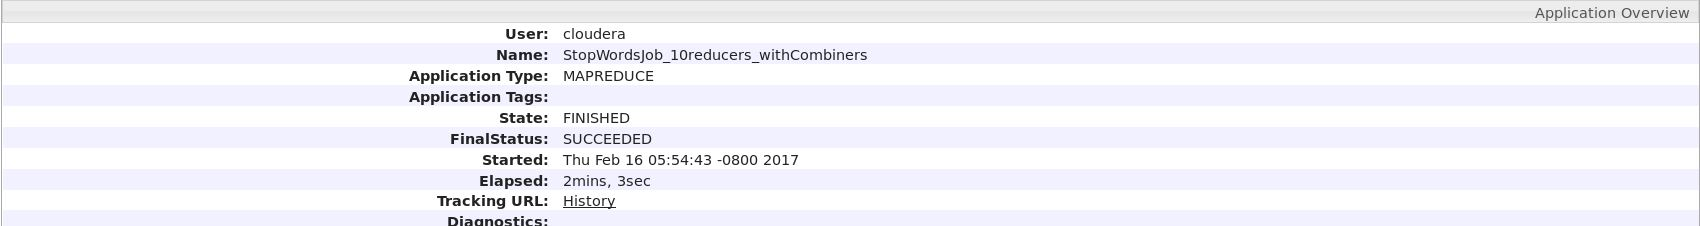
\includegraphics[keepaspectratio=true,width=\dimmin{}{\dimwidth{1.30}}]{images/stopwords3}{}

\noindent There is a difference in execution time as the program with combiner takes 32 seconds less.%mdk

The Combiner is a semi-reducer.The Combiner class is used in between the Map class and 
the Reduce class to reduce the volume of data transfer between Mapper and Reducer.It does a partial reduction at the map nodes before transfering the data to the reduction phase.
Since Reduction cannot perform parallelization but the mapper can, the combiner decreases the data to be reduced by the Reducer class and thus leads to a decrease in execution time.%mdk

\subsubsection{2.1.3.\hspace*{0.5em}Run the same program again, this time compressing the intermediate results of map (using any codec you wish). Report the execution time. Is there any difference in the execution, time compared to the previous execution? Why?}\label{heading}%mdk%mdk

\noindent We run the same program in 2.1.2 but add  the following code in the configuration class:%mdk
\begin{mdpre}%mdk
\noindent FileOutputFormat.setCompressOutput(job,~{\mdcolor{navy}true});\\
~~~~~~~~FileOutputFormat.setOutputCompressorClass(job,\\
~~~~~~~~~~~~~~~~org.apache.hadoop.io.compress.BZip2Codec.{\mdcolor{navy}class});%mdk
\end{mdpre}\noindent The BZip2 codec has been chosen for this instance. bzip2 is a free and open-source file compression program that uses the Burrows–Wheeler algorithm. It only compresses single files and is not a file archiver. 
It compresses data in blocks of size between 100 and 900 kB and uses the Burrows–Wheeler transform to convert frequently-recurring character sequences into strings of identical letters. It then applies move-to-front transform and Huffman coding.
There are other codecs which can be used like: Snappy, LZO , GZip. BZip2, LZO, and Snappy formats are splittable, but GZip is not.

Execution Time:
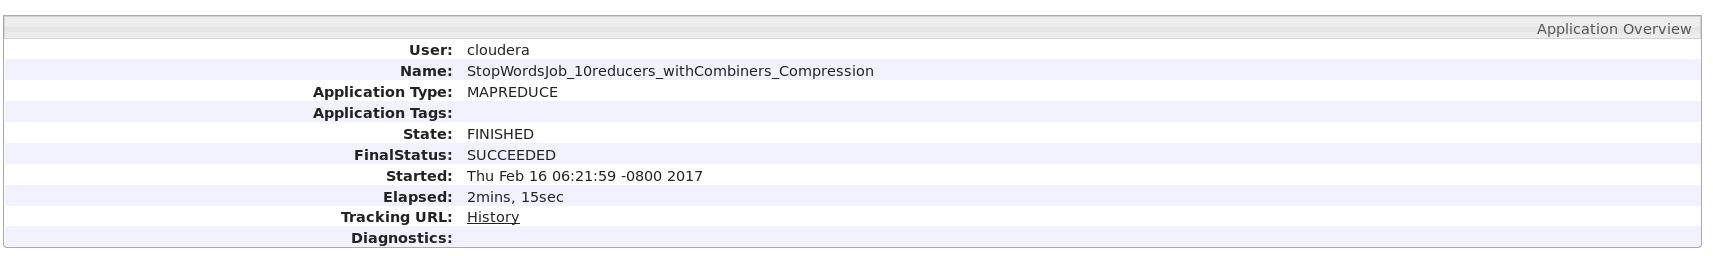
\includegraphics[keepaspectratio=true,width=\dimmin{}{\dimwidth{1.30}}]{images/stopwords4}{}%mdk

\noindent There is a slight increase of 13 seconds in the execution time which is due to the time taken for compression.%mdk

\subsubsection{2.1.4.\hspace*{0.5em}Run the same program again, this time using 50 reducers. Report the execution time. Is there any difference in the execution time, compared to the previous execution? Why?}\label{heading}%mdk%mdk

\noindent We make the following change to the code in 2.1.3%mdk
\begin{mdpre}%mdk
\noindent job.setNumReduceTasks({\mdcolor{purple}50});%mdk
\end{mdpre}\noindent Execution Time:
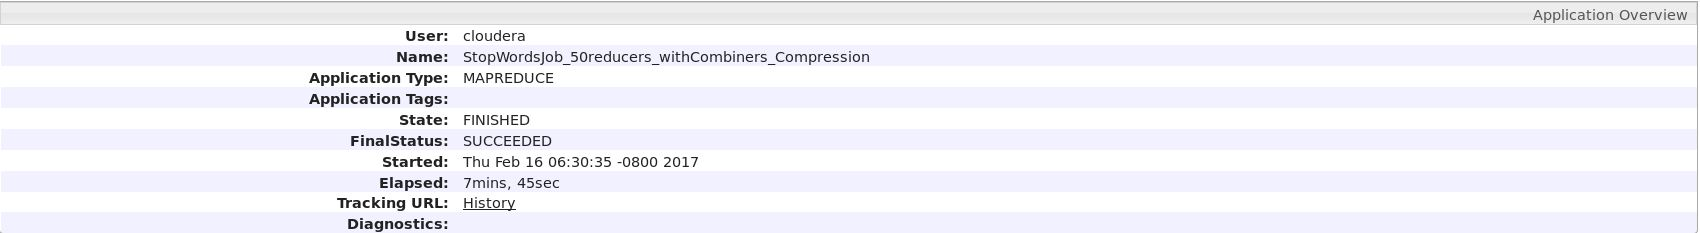
\includegraphics[keepaspectratio=true,width=\dimmin{}{\dimwidth{1.30}}]{images/stopwords5}{}

\noindent There is a huge difference compared to the execution time. As there are 50 reducers and since Reducers dont implement parallelization, it takes lot more time to run 50 of them and also having compression done too.%mdk

\subsection{2.2.\hspace*{0.5em}Question: Inverted Index}\label{heading}%mdk%mdk

\subsubsection{2.2.1.\hspace*{0.5em}Implement a simple inverted index for the given document corpus, as shown in the previous Table, skipping the words of stopwords.csv}\label{heading}%mdk%mdk

\noindent Now, we have to make changes to the Map class for this. Since it is an inverted index, for each word in the corpus
the program needs to generate the output : (word,list of file names).
So we set both key and value to Text class.%mdk
\begin{mdpre}%mdk
\noindent job.setOutputKeyClass(Text.{\mdcolor{navy}class});\\
~~~~~~~~job.setOutputValueClass(Text.{\mdcolor{navy}class});%mdk
\end{mdpre}\noindent Now our program needs to not only create the inverted index but also create it without using the words in the stopwords list.
Thus we need to read the words from the stopwords.csv file. The stopwords.csv has been converted into stopwords.txt to make it simpler to execute:
\begin{mdpre}%mdk
\noindent a\\
about\\
after\\
again\\
all%mdk
\end{mdpre}\noindent We also changed the output config format from csv :
\begin{mdpre}%mdk
\noindent job.getConfiguration().set(\\
~~~~~~~~~~~~~~~~{\mdcolor{maroon}"}{\mdcolor{maroon}mapreduce.output.textoutputformat.separator}{\mdcolor{maroon}"},~{\mdcolor{maroon}"}{\mdcolor{maroon}~-\textgreater{}~}{\mdcolor{maroon}"});%mdk
\end{mdpre}\noindent We use the FileSplit function to get the filenames and the String Tokenizer to split. The BufferedReader creates Reader object to read from the \textquotedblleft{}stopwords.txt\textquotedblright{} file. The following is the mapper class code:
\begin{mdpre}%mdk
\noindent{\mdcolor{navy}public}~{\mdcolor{navy}static}~{\mdcolor{navy}class}~StubMapper~{\mdcolor{navy}extends}~Mapper\textless{}LongWritable,~Text,~Text,~Text\textgreater{}~\{\\
~~~~~~~~{\mdcolor{navy}private}~Text~word~=~{\mdcolor{navy}new}~Text();\\
~~~~~~~~{\mdcolor{navy}private}~Text~filename~=~{\mdcolor{navy}new}~Text();\\
\\
~~~~~~~~@Override\\
~~~~~~~~{\mdcolor{navy}public}~{\mdcolor{navy}void}~map(LongWritable~key,~Text~value,~Context~context)\\
~~~~~~~~~~~~~~~~{\mdcolor{navy}throws}~IOException,~InterruptedException~\{\\
~~~~~~~~~~~~HashSet\textless{}String\textgreater{}~stopwords~=~{\mdcolor{navy}new}~HashSet\textless{}String\textgreater{}();\\
~~~~~~~~~~~~BufferedReader~Reader~=~{\mdcolor{navy}new}~BufferedReader(\\
~~~~~~~~~~~~~~~~~~~~{\mdcolor{navy}new}~FileReader(\\
~~~~~~~~~~~~~~~~~~~~~~~~~~~~{\mdcolor{navy}new}~File(\\
~~~~~~~~~~~~~~~~~~~~~~~~~~~~~~~~~~~~{\mdcolor{maroon}"}{\mdcolor{maroon}/home/cloudera/workspace/MDP\_Assignment1/stopwords.txt}{\mdcolor{maroon}"})));\\
~~~~~~~~~~~~String~line;\\
~~~~~~~~~~~~{\mdcolor{navy}while}~((line~=~Reader.readLine())~!=~{\mdcolor{navy}null})~\{\\
~~~~~~~~~~~~~~~~stopwords.add(line.{\mdcolor{navy}toString}().toLowerCase());\\
~~~~~~~~~~~~\}\\
~~~~~~~~~~~~Reader.close();\\
~~~~~~~~~~~~String~filenameStr~=~((FileSplit)~context.getInputSplit()).getPath().getName();~~~~~~~~~~~~\\
~~~~~~~~~~~~filename~=~{\mdcolor{navy}new}~Text(filenameStr);\\
~~~~~~~~~~~~StringTokenizer~tokenizer~=~{\mdcolor{navy}new}~StringTokenizer(value.{\mdcolor{navy}toString}().replaceAll({\mdcolor{maroon}"}{\mdcolor{maroon}{}[}{\mdcolor{gray}\textbackslash{}\textbackslash{}}{\mdcolor{maroon}p\{Punct\}}{\mdcolor{gray}\textbackslash{}\textbackslash{}}{\mdcolor{maroon}d~]}{\mdcolor{maroon}"},{\mdcolor{maroon}"}{\mdcolor{maroon}~}{\mdcolor{maroon}"}));\\
~~~~~~~~~~~~{\mdcolor{darkgreen}//System.out.print(tokenizer);}\\
~~~~~~~~~~~~{\mdcolor{navy}while}~(tokenizer.hasMoreTokens())~\{\\
~~~~~~~~~~~~~~~~word.set(tokenizer.nextToken().{\mdcolor{navy}toString}().toLowerCase());~~~~\\
~~~~~~~~~~~~~~~~context.write(word,filename);\\
~~~~~~~~~~~~\}~~~~\\
~~~~~~~~\}\\
~~~~\}%mdk
\end{mdpre}\noindent The above mapper class will give  a (key, value) pair output of the form (word, filename):
\begin{mdpre}%mdk
\noindent word1,~doc1.txt\\
word1,~doc1.txt\\
word1,~doc1.txt\\
word1,~doc2.txt\\
word2,~doc1.txt\\
word2,~doc2.txt\\
word2,~doc2.txt\\
word2,~doc3.txt%mdk
\end{mdpre}\noindent The following reducer class then stores all the values of the filenames for each word in a HashSet. The HashSet is used to avoid duplicates in case of the words.
\begin{mdpre}%mdk
\noindent~~~~{\mdcolor{navy}public}~{\mdcolor{navy}static}~{\mdcolor{navy}class}~StubReducer~{\mdcolor{navy}extends}~Reducer\textless{}Text,~Text,~Text,~Text\textgreater{}~\{\\
\\
~~~~~~~~@Override\\
~~~~~~~~{\mdcolor{navy}public}~{\mdcolor{navy}void}~reduce(Text~key,~Iterable\textless{}Text\textgreater{}~values,~Context~context)\\
~~~~~~~~~~~~~~~~{\mdcolor{navy}throws}~IOException,~InterruptedException~\{\\
~~~~~~~~~~~~HashSet\textless{}String\textgreater{}~rehash~=~{\mdcolor{navy}new}~HashSet\textless{}String\textgreater{}();\\
~~~~~~~~~~~~{\mdcolor{navy}for}~(Text~value~:~values)~\{\\
~~~~~~~~~~~~~~~~rehash.add(value.{\mdcolor{navy}toString}());\\
~~~~~~~~~~~~\}\\
~~~~~~~~~~~~StringBuilder~builder~=~{\mdcolor{navy}new}~StringBuilder();\\
~~~~~~~~~~~~String~prefix~=~{\mdcolor{maroon}"}{\mdcolor{maroon},~}{\mdcolor{maroon}"};\\
~~~~~~~~~~~~{\mdcolor{navy}for}~(String~value~:~rehash)~\{\\
~~~~~~~~~~~~~~~~builder.append(prefix);\\
~~~~~~~~~~~~~~~~builder.append(value);\\
~~~~~~~~~~~~\}\\
~~~~~~~~~~~~context.write(key,~{\mdcolor{navy}new}~Text(builder.{\mdcolor{navy}toString}()));\\
~~~~~~~~\}\\
~~~~\}%mdk
\end{mdpre}\noindent The Reducer class gives a  output of the form (word, collection of filenames) in the following format:
\begin{mdpre}%mdk
\noindent a~-\textgreater{}~pg31100.txt,~pg3200.txt,~pg100.txt\\
aachen~-\textgreater{}~pg3200.txt\\
aar~-\textgreater{}~pg3200.txt\\
aaron~-\textgreater{}~pg3200.txt,~pg100.txt%mdk
\end{mdpre}\noindent Execution Time:
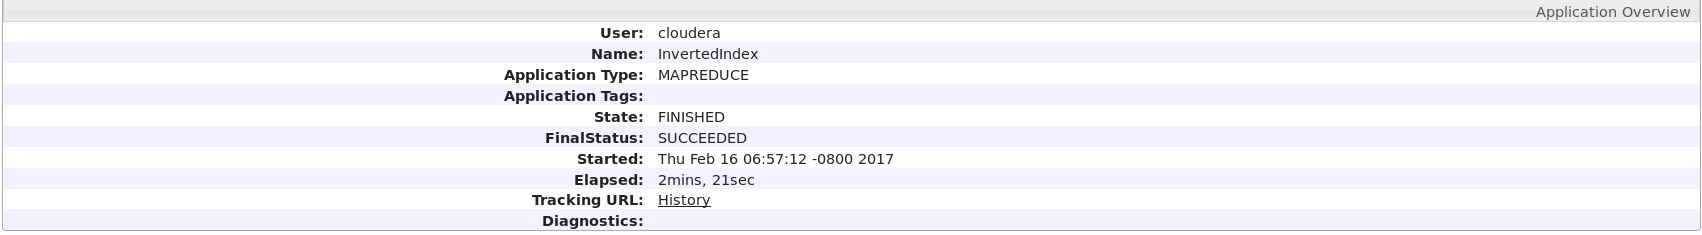
\includegraphics[keepaspectratio=true,width=\dimmin{}{\dimwidth{1.30}}]{images/invertedindex}{}

\subsubsection{2.2.2.\hspace*{0.5em}How many unique words exist in the document corpus (excluding stop words)? Which counter(s) reveal(s) this information? Define your own counter for the number of words appearing in a single document only. What is the value of this counter? Store the final value of this counter on a new file on HDFS.}\label{heading}%mdk%mdk

\noindent We first add the following counter to the previous program in 2.2.1 :%mdk
\begin{mdpre}%mdk
\noindent{\mdcolor{navy}public}~{\mdcolor{navy}static}~{\mdcolor{navy}enum}~COUNTER~\{\\
~~~~~~~~UniqueWords,\\
~~~~\};%mdk
\end{mdpre}\noindent The mapper function will remain the same as we are not doing further selective mapping. We will have to make changes to our reuducer function so that only unique words are selected. 
UniqueWords are the words which are present in only one file and not in multiple ones. Thus the size of filelist for such words will be 1.

The following is our Reducer Class:
There is a if statement which only count the words whose filename size is 1. The increment function increments the counter by 1 for every unique word.%mdk
\begin{mdpre}%mdk
\noindent{\mdcolor{navy}public}~{\mdcolor{navy}static}~{\mdcolor{navy}class}~StubReducer~{\mdcolor{navy}extends}~Reducer\textless{}Text,~Text,~Text,~Text\textgreater{}~\{\\
\\
~~~~~~~~@Override\\
~~~~~~~~{\mdcolor{navy}public}~{\mdcolor{navy}void}~reduce(Text~key,~Iterable\textless{}Text\textgreater{}~values,~Context~context)\\
~~~~~~~~~~~~~~~~{\mdcolor{navy}throws}~IOException,~InterruptedException~\{\\
~~~~~~~~~~~~HashSet\textless{}String\textgreater{}~rehash~=~{\mdcolor{navy}new}~HashSet\textless{}String\textgreater{}();\\
~~~~~~~~~~~~{\mdcolor{navy}for}~(Text~value~:~values)~\{\\
~~~~~~~~~~~~~~~~rehash.add(value.{\mdcolor{navy}toString}());\\
~~~~~~~~~~~~\}\\
~~~~~~~~~~~~{\mdcolor{navy}if}~(rehash.size()~==~{\mdcolor{purple}1})~\{\\
~~~~~~~~~~~~~~~~context.getCounter(COUNTER.UniqueWords).increment({\mdcolor{purple}1});\\
~~~~~~~~~~~~StringBuilder~builder~=~{\mdcolor{navy}new}~StringBuilder();\\
~~~~~~~~~~~~String~prefix~=~{\mdcolor{maroon}"}{\mdcolor{maroon},~}{\mdcolor{maroon}"};\\
~~~~~~~~~~~~{\mdcolor{navy}for}~(String~value~:~rehash)~\{\\
~~~~~~~~~~~~~~~~builder.append(prefix);\\
~~~~~~~~~~~~~~~~builder.append(value);\\
~~~~~~~~~~~~\}\\
~~~~~~~~~~~~context.write(key,~{\mdcolor{navy}new}~Text(builder.{\mdcolor{navy}toString}()));\\
~~~~~~~~\}\\
~~~~~~~~\}\\
~~~~\}%mdk
\end{mdpre}\noindent After executing the Hadoop Job: We can see the Counter details in the job summary:-
\begin{mdpre}%mdk
\noindent hadoop~jar~MDP\_Assignment1.jar~invertedindex.InvertedIndexUnique~input~output\\
{\mdcolor{darkgreen}//in~the~job~summary~~}\\
~~invertedindex.InvertedIndexUnique\$COUNTER\\
~~~~~~~~UniqueWords={\mdcolor{purple}35726}%mdk
\end{mdpre}\noindent Execution Time:
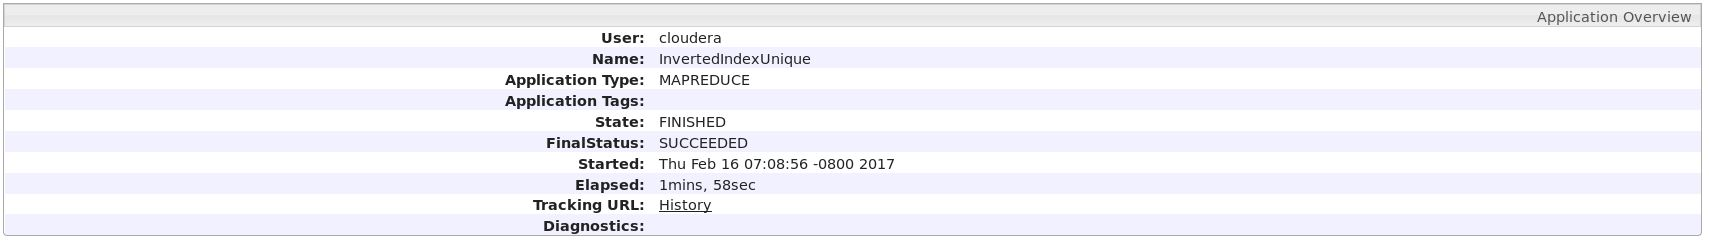
\includegraphics[keepaspectratio=true,width=\dimmin{}{\dimwidth{1.30}}]{images/iiunique}{}

\subsubsection{2.2.3.\hspace*{0.5em}Extend the inverted index of (b), in order to keep the frequency of each word for each document. The new output should be of the form:}\label{sec-extend-the-inverted-index-of-b-in-order-to-keep-the-frequency-of-each-word-for-each-document-the-new-output-should-be-of-the-form-}%mdk%mdk
\begin{mdtabular}{2}{\dimeval{(\linewidth)/2}}{1ex}%mdk
\begin{tabular}{lc}\midrule
\multicolumn{1}{|c}{{\bfseries word}}&\multicolumn{1}{c|}{{\bfseries Filename and Frequency}}\\

\midrule
\multicolumn{1}{|l}{this}&\multicolumn{1}{c|}{doc1.txt\#1, doc2.txt\#1}\\
\multicolumn{1}{|l}{is}&\multicolumn{1}{c|}{doc1.txt\#2, doc2.txt\#1, doc3.txt\#1}\\
\midrule
\end{tabular}\end{mdtabular}

\noindent which means that the word frequency should follow a single ‘\#’ character, which should follow the filename, for each file that contains this word. You are required to use a Combiner.%mdk

In this case we can extend the Mapper function from the previous program with the only difference being:%mdk
\begin{mdpre}%mdk
\noindent{\mdcolor{navy}public}~{\mdcolor{navy}static}~{\mdcolor{navy}class}~StubMapper~{\mdcolor{navy}extends}~Mapper\textless{}Object,~Text,~Text,~Text\textgreater{}~\{\\
~~~~~~~~{\mdcolor{navy}private}~Text~word~=~{\mdcolor{navy}new}~Text();\\
~~~~~~~~{\mdcolor{navy}private}~Text~filename~=~{\mdcolor{navy}new}~Text();\\
\\
~~~~~~~~@Override\\
~~~~~~~~{\mdcolor{navy}public}~{\mdcolor{navy}void}~map(Object~key,~Text~value,~Context~context)%mdk
\end{mdpre}\noindent Now, we have to use a combiner which will partially reduce the function before it is passed onto the actual reducer. 
The combiner extends the reducer class. The Reducer class is as follows:
\begin{mdpre}%mdk
\noindent{\mdcolor{navy}public}~{\mdcolor{navy}static}~{\mdcolor{navy}class}~StubReducer~{\mdcolor{navy}extends}~Reducer\textless{}Text,~Text,~Text,~Text\textgreater{}~\{\\
~~~~{\mdcolor{navy}private}~~Text~combo={\mdcolor{navy}new}~Text();~{\mdcolor{darkgreen}//~takes~the~combination~of~filename~and~frequency}\\
~~~~~~~~@Override\\
~~~~~~~~{\mdcolor{navy}public}~{\mdcolor{navy}void}~reduce(Text~key,~Iterable\textless{}Text\textgreater{}~values,~Context~context)\\
~~~~~~~~~~~~~~~~{\mdcolor{navy}throws}~IOException,~InterruptedException~\{\\
~~~~~~~~~~~~String~result={\mdcolor{navy}new}~String();\\
~~~~~~~~~~~~Map\textless{}String,Integer\textgreater{}~nmap={\mdcolor{navy}new}~HashMap\textless{}String,Integer\textgreater{}();~{\mdcolor{darkgreen}//map~the~dataset}\\
~~~~~~~~~~~~String~Filename={\mdcolor{navy}new}~String();\\
~~~~~~~~~~~~Integer~count={\mdcolor{navy}new}~Integer({\mdcolor{purple}0});\\
~~~~~~~~~~~~{\mdcolor{navy}for}~(Text~value~:~values)~\{\\
~~~~~~~~~~~~~~~~String{}[]~s=value.{\mdcolor{navy}toString}().split({\mdcolor{maroon}"}{\mdcolor{maroon}\#}{\mdcolor{maroon}"});\\
~~~~~~~~~~~~~~~~Filename=s{}[{\mdcolor{purple}0}];\\
~~~~~~~~~~~~~~~~count={\mdcolor{navy}new}~Integer(s{}[{\mdcolor{purple}1}]);\\
~~~~~~~~~~~~~~~~{\mdcolor{navy}if}(nmap.containsKey(Filename))\\
~~~~~~~~~~~~~~~~\{\\
~~~~~~~~~~~~~~~~~~~~nmap.put(Filename,~nmap.get(Filename)+count);~~~~~\\
~~~~~~~~~~~~~~~~\}\\
~~~~~~~~~~~~~~~~{\mdcolor{navy}else}\\
~~~~~~~~~~~~~~~~\{\\
~~~~~~~~~~~~~~~~~~~~nmap.put(Filename,~count);\\
~~~~~~~~~~~~~~~~\}\\
~~~~~~~~~~~~\}\\
~~~~~~~~~~~~{\mdcolor{navy}for}~(String~v~:nmap.keySet())~\\
~~~~~~~~~~~~\{~~~~\\
~~~~~~~~~~~~~result+={\mdcolor{maroon}"}{\mdcolor{maroon},}{\mdcolor{maroon}"}+v+{\mdcolor{maroon}"}{\mdcolor{maroon}\#}{\mdcolor{maroon}"}+nmap.get(Filename).{\mdcolor{navy}toString}();\\
~~~~~~~~~~~~\}\\
~~~~~combo.set(result);\\
~~~~~~~~~context.write(key,~combo);\\
\\
~~~~~~~~\}\\
~~~~\}%mdk
\end{mdpre}\noindent The Combiner Class is as follows:
\begin{mdpre}%mdk
\noindent{\mdcolor{navy}public}~{\mdcolor{navy}static}~{\mdcolor{navy}class}~StubCombiner~{\mdcolor{navy}extends}~Reducer\textless{}Text,Text,Text,Text\textgreater{}\\
~~~~\{~~~{\mdcolor{navy}private}~Text~combo=~{\mdcolor{navy}new}~Text();\\
~~~~~~~~{\mdcolor{navy}public}~{\mdcolor{navy}void}~reduce(Text~key,~Iterable\textless{}Text\textgreater{}~values,~Context~context)~{\mdcolor{darkgreen}//Iterable~to~count~the~frequency}\\
~~~~~~~~~~~~~~~~{\mdcolor{navy}throws}~IOException,~InterruptedException~\{~~~~\\
~~~~~~~~~~~~Integer~frequency={\mdcolor{navy}new}~Integer({\mdcolor{purple}0});\\
~~~~~~~~~~~~String~fname=~{\mdcolor{navy}new}~String();\\
~~~~~~~~~~~~\\
~~~~~~~~~~~~{\mdcolor{navy}for}(Text~val:values)\\
~~~~~~~~~~~~\{\\
~~~~~~~~~~~~~~~~frequency=frequency+{\mdcolor{purple}1};~~~{\mdcolor{darkgreen}//for~each~word~in~a~document~increment~the~frequency}\\
~~~~~~~~~~~~~~~~{\mdcolor{navy}if}(frequency=={\mdcolor{purple}1})\\
~~~~~~~~~~~~~~~~\{\\
~~~~~~~~~~~~~~~~~~~~fname=val.{\mdcolor{navy}toString}();~~~~~~~~~~~~~~~~\\
~~~~~~~~~~~~~~~~\}~~~~\\
~~~~~~~~~~~~\}\\
~~~~~~~~~~~~combo.set(fname+{\mdcolor{maroon}"}{\mdcolor{maroon}\#}{\mdcolor{maroon}"}+frequency.{\mdcolor{navy}toString}());~~{\mdcolor{darkgreen}//joining~the~document~and~frequency}\\
~~~~~~~~~~~~context.write(key,combo);~\\
~~~~~~~~\}\\
~~~~\}%mdk
\end{mdpre}\noindent The logic behind using the combiner is to have partial reduction at the Mapper phase thus reducing the workload for the reducer class.
The output csv file is as follows:
\begin{mdpre}%mdk
\noindent a~-\textgreater{}~,pg31100.txt\#{\mdcolor{purple}73628},pg3200.txt\#{\mdcolor{purple}73628},pg100.txt\#{\mdcolor{purple}73628}\\
aachen~-\textgreater{}~,pg3200.txt\#{\mdcolor{purple}1}\\
aar~-\textgreater{}~,pg3200.txt\#{\mdcolor{purple}3}\\
aaron~-\textgreater{}~,pg3200.txt\#{\mdcolor{purple}97},pg100.txt\#{\mdcolor{purple}97}%mdk
\end{mdpre}\noindent Execution Time:

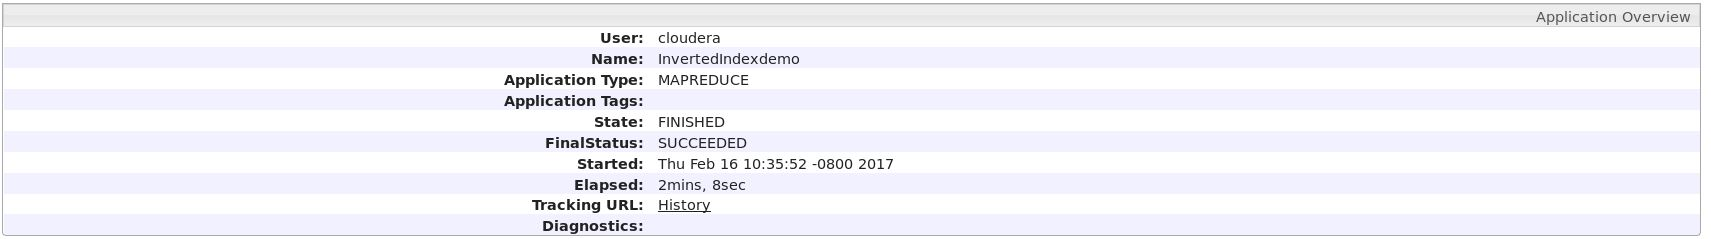
\includegraphics[keepaspectratio=true,width=\dimmin{}{\dimwidth{1.30}}]{images/iifreq}{}%mdk

\section{3.\hspace*{0.5em}CONCLUSION}\label{heading}%mdk%mdk

\noindent The overview of the Stopwords portion of the assignment:%mdk
\begin{mdtabular}{2}{\dimeval{(\linewidth)/2}}{1ex}%mdk
\begin{tabular}{lc}\midrule
\multicolumn{1}{|c}{{\bfseries Method}}&\multicolumn{1}{c|}{{\bfseries Runtime (in secs)}}\\

\midrule
\multicolumn{1}{|l}{Stopwords}&\multicolumn{1}{c|}{108}\\
\multicolumn{1}{|l}{10 Reducers and no combiners}&\multicolumn{1}{c|}{155}\\
\multicolumn{1}{|l}{10 Reducers and a combiner}&\multicolumn{1}{c|}{123}\\
\multicolumn{1}{|l}{10 Reducers,combiner,compression}&\multicolumn{1}{c|}{135}\\
\multicolumn{1}{|l}{50 Reducers,combiner,compression}&\multicolumn{1}{c|}{465}\\
\midrule
\end{tabular}\end{mdtabular}

\noindent We can conclude that due to lack of parallelization in case of a Reducer, the higher the number of reducers the larger is the
execution time. Compression also affects the execution time depending on the type(codec). Combiners are used for optimizing and thus reduces the execution time.%mdk

The Runtime Overview of the InvertedIndex jobs:%mdk
\begin{mdtabular}{2}{\dimeval{(\linewidth)/2}}{1ex}%mdk
\begin{tabular}{lc}\midrule
\multicolumn{1}{|c}{{\bfseries Method}}&\multicolumn{1}{c|}{{\bfseries Runtime(in secs)}}\\

\midrule
\multicolumn{1}{|l}{Inverted Index Simple}&\multicolumn{1}{c|}{141}\\
\multicolumn{1}{|l}{Inverted Index Unique Words}&\multicolumn{1}{c|}{118}\\
\multicolumn{1}{|l}{Inverted Index Word Frequency using Custom Combiner}&\multicolumn{1}{c|}{128}\\
\midrule
\end{tabular}\end{mdtabular}

\noindent The Inverted Index jobs were simple version of what can be used in search engine implementation and optimization. Even though 
the Inverted Index with Frequency has more complexity than the simple Inverted Index job, the use of a combiner reduces the runtime.%mdk%mdk


\end{document}
